\documentclass[11pt]{article}

% Libraries.
\usepackage{amsmath}
\usepackage{amssymb}
\usepackage{pgfplots}
\usepackage{graphicx}
\usepackage{enumitem}
\usepackage{hyperref}
\usepackage{fancyhdr}
\usepackage{perpage}
\usepackage{float}
\usepackage{esint}

% Property settings.
\MakePerPage{footnote}
\pagestyle{headings}

% Commands
\newcommand{\ti}[1]{\textit{#1}}
\newcommand{\tb}[1]{\textbf{#1}}
\newcommand{\mb}[1]{\mathbb{#1}}
\newcommand{\bx}[0]{\mathbf{x}}
\newcommand{\bv}[0]{\mathbf{v}}
\newcommand{\bw}[0]{\mathbf{w}}
\newcommand{\real}[0]{\mathbb{R}}
\newcommand{\under}[1]{\underline{#1}}
\newcommand{\proof}[0]{\textit{\underline{proof:} }}
\newcommand{\func}[3]{\tb{#1}: {#2} \rightarrow {#3} }
\newcommand{\vx}[0]{\tb{x}}
\newcommand{\vy}[0]{\tb{y}}
\newcommand{\vz}[0]{\tb{z}}
\newcommand{\vo}[0]{\tb{0}}
\newcommand{\va}[0]{\tb{a}}
\newcommand{\vb}[0]{\tb{b}}
\newcommand{\vc}[0]{\tb{c}}
\newcommand{\ve}[0]{\tb{e}}
\newcommand{\vm}[0]{\tb{m}}
\newcommand{\vh}[0]{\tb{h}}
\newcommand{\vf}[0]{\tb{F}}
\newcommand{\vi}[0]{\tb{i}}
\newcommand{\vj}[0]{\tb{j}}
\newcommand{\vk}[0]{\tb{k}}
\newcommand{\vg}[0]{\tb{G}}
\newcommand{\vn}[0]{\tb{n}}
\newcommand{\vu}[0]{\tb{u}}
\newcommand{\vv}[0]{\tb{v}}
\newcommand{\vL}[0]{\tb{L}}
\newcommand{\ff}[0]{\tb{f}}
\newcommand{\fg}[0]{\tb{g}}
\newcommand{\p}[0]{\partial}
\newcommand{\qed}[0]{$\hfill\blacksquare$}
\newcommand{\qerat}{\tag*{$\blacksquare$}}
\newcommand{\lima}{\underset{\vx \rightarrow \va}{\lim}}
\usepackage{amsmath}% http://ctan.org/pkg/amsmath
\newcommand{\notimplies}{%
  \mathrel{{\ooalign{\hidewidth$\not\phantom{=}$\hidewidth\cr$\implies$}}}}
\newcommand{\q}[0]{\textcolor{red}{???}}
% Attr.
\title{APM462 \\ Lecture Notes}
\author{Yuchen Wang}
\date{\today}

\begin{document}
    \maketitle
    \tableofcontents
    \newpage
    
\section{Matrix Calculus}
\paragraph{Row v.s. Column Vector}
Our default rule is that every vector is a column vector unless explicitly stated otherwise. \\
This is also known as the \under{numerator layout}. \\
\under{Special case}: For $f: \real^n \rightarrow \real$, $Df$ is a $ 1 \times n$ matrix or row vector.

\subsection{Matrix Multiplication}
\paragraph{Definition 1.1.1}
Let A be $m \times n$, and B be $n \times p$, and let the product AB be
$$C = AB$$
then $C$ is a $m \times p$ matrix, with element $(i,j)$ given by
$$c_{ij} = \sum_{k=1}^n a_{ik}b_{kj}$$
for all $i = 1, 2, \hdots, m, j = 1,2,\hdots,p$.
\paragraph{Proposition 1.1.2}
Let $A$ be $m \times n$, and $x$ be $n \times 1$, then the typical element of the product
$$ z = Ax$$
is given by
$$z_i = \sum_{k=1}^n a_{ik}x_k$$
for all $i= 1,2,\hdots,m$.\\
Similarly, let $y$ be $m \times 1$, then the typical element of the product
$$z^T = y^TA$$
is given by
$$ z_i = \sum_{k=1}^n a_{ki}y_k$$
for all $i = 1, 2,\hdots, n$.  \\
Finally, the scalar resulting from the product
$$\alpha = y^T A x$$
is given by
$$\alpha = \sum_{j=1}^m\sum_{k=1}^n a_{jk}y_i x_k$$

\subsection{Partitioned Matrices}
\paragraph{Proposition 1.2.1}
Let $A$ be a square, nonsingular matrix of order $m$. Partition A as
$$ A = \begin{bmatrix}
	A_{11} & A_{12} \\
	A_{21} & A_{22}
\end{bmatrix}
$$
so that $A_{11}$ and $A_{22}$ are invertible. \\
Then
$$ A^{-1} = \begin{bmatrix}
	(A_{11} - A_{12}A_{22}^{-1}A_{21})^{-1} & -A_{11}^{-1}A_{12}(A_{22} - A_{21}A_{11}^{-1}A_{12})^{-1} \\
	-A_{22}^{-1}A_{21}(A_{11} - A_{12}A_{22}^{-1}A_{21})^{-1} & (A_{22} - A_{21}A_{11}^{-1}A_{12})^{-1}
\end{bmatrix}$$
\proof \\
Direct multiplication of the proposed $A^{-1}$ and $A$ yields
$$A^{-1}A = I$$ \qed

\subsection{Matrix Differentiation}
\paragraph{Proposition 1.3.1}
$$\frac{\partial A}{\partial x} = \frac{\partial A^T}{\partial x}$$
\paragraph{Proposition 1.3.2}
Let $$y = Ax$$
where $y$ is $m\times 1$, $x$ is $n \times 1$, A is $m \times n$, and $A$ does not depend on $x$. Suppose that $x$ is a function of the vector $z$, while $A$ is independent of $z$. Then
$$\frac{\partial y }{\partial z} = A \frac{\partial x}{\partial z}$$

\paragraph{Proposition 1.3.3}
Let the \textcolor{red}{scalar} $\alpha$ be defined by
$$\alpha = y^T Ax$$
where $y$ is $m \times 1$, $x$ is $n \times 1$, $A$ is $m \times n$, and $A$ is independent of $x$ and $y$, then
$$\frac{\partial \alpha}{\partial x} = y^TA$$
and 
$$\frac{\partial \alpha}{\partial y} = x^TA^T$$

\paragraph{Proposition 1.3.4}
For the special case where the \textcolor{red}{scalar} $\alpha$ is given by the quadratic form
$$\alpha = x^TAx$$
where $x$ is $n \times 1$, $A$ is $n \times n$, and $A$ does not depend on $x$, then
$$\frac{\partial \alpha}{\partial x} = x^T (A + A^T)$$
\proof \\
By definition
$$\alpha = \sum_{j=1}^n \sum_{i=1}^n a_{ij}x_ix_j$$
Differentiating with respect to the $k$th element of $x$ we have
$$\frac{\partial \alpha}{\partial x_k} = \sum_{j=1}^n a_{kj}x_J + \sum_{i=1}^n a_{ik}x_i$$
for all $k = 1,2, \hdots, n$, and consequently,
$$\frac{\partial \alpha}{\partial x} = x^TA^T + x^TA = x^T(A^T + A)$$ \qed

\paragraph{Proposition 1.3.4}
For the special case where \textcolor{red}{$A$ is a symmetric matrix} and
$$\alpha = x^TAx$$
where $x$ is $n \times 1$, $A$ is $n \times n$, and $A$ does not depend on $x$, then
$$\frac{\partial \alpha}{\partial x} = 2x^TA$$

\paragraph{Proposition 1.3.5}
Let the \textcolor{red}{scalar} $\alpha$ be defined by
$$\alpha = y^Tx$$
where $y$ is $n \times 1$, $x$ is $n \times 1$, and both $y$ and $x$ are functions of the vector $z$. Then
$$\frac{\partial \alpha}{\partial z} = x^T \frac{\partial y}{\partial z} + y^T \frac{\partial x}{\partial z}$$

\paragraph{Proposition 1.3.6}
Let the \textcolor{red}{scalar} $\alpha$ be defined by
$$\alpha = x^Tx$$
where $x$ is $n \times 1$, and $x$ is a functions of the vector $z$. Then
$$\frac{\partial \alpha}{\partial z} = 2x^T \frac{\partial y}{\partial z}$$

\paragraph{Proposition 1.3.7}
Let the \textcolor{red}{scalar} $\alpha$ be defined by
$$\alpha = y^TAx$$
where $y$ is $m \times 1$, $A$ is $m \times n$, $x$ is $n \times 1$, and both $y$ and $x$ are functions of the vector $z$, while $A$ does not depend on $z$. Then
$$\frac{\partial \alpha}{\partial z} = x^T A^T\frac{\partial y}{\partial z} + y^T A\frac{\partial x}{\partial z}$$

\paragraph{Proposition 1.3.8}
Let $A$ be an invertible, $m \times m$ matrix whose elements are functions of the scalar parameter $\alpha$. Then
$$\frac{\partial A^{-1}}{\partial \alpha} = -A^{-1}\frac{\partial A}{\partial \alpha} A^{-1}$$
\proof \\
Start with the definition of the inverse
$$A^{-1}A = I$$
and differentiate, yielding
$$A^{-1}\frac{\partial A}{\partial \alpha} + \frac{\partial A^{-1}}{\partial \alpha}A = 0$$
rearranging the terms yields
$$\frac{\partial A^{-1}}{\partial \alpha}  = -A^{-1}\frac{\partial A}{\partial \alpha}A^{-1}$$\qed

\paragraph{Vector-by-vector Differentiation Identities 1.3.9}
 \begin{figure}[h]
	\centering
	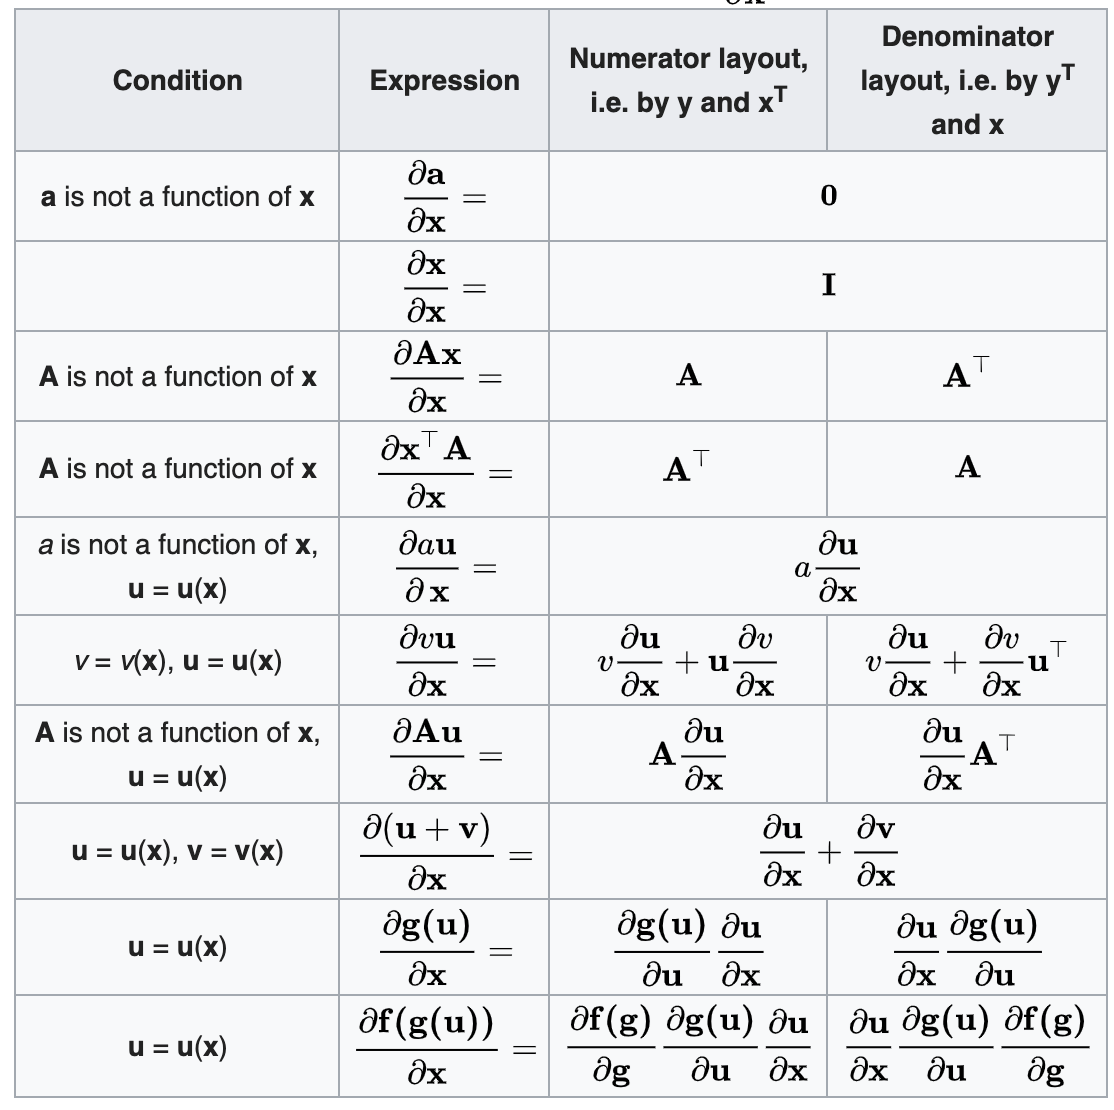
\includegraphics[scale=0.6]{p1.png}
\end{figure}

\paragraph{Young's Theorem 1.3.10}
i.e. Symmetry of second derivatives
$$[\nabla_{xy}f(x,y)]^T = \nabla_{yx}f(x,y)$$
\proof \\
This is straightforward by writing out the elements of the matrix. \qed


\section{Second-year Calculus Review}
functions $\real \rightarrow \real$
\subsection{Mean Value Theorem in 1 Dimension}
$g \in C^1$ on $\real$
$$\frac{g(x+h) - g(x)}{h} = g'(x + \theta h)$$
where $\theta \in (0,1)$ \\
Or equivalently,
$$g(x+h) = g(x) + hg'(x+\theta h)$$

\subsection{1st Order Taylor Approximation}
$g \in C^1$ on $\real$
$$g(x + h) = g(x) + hg'(x) + o(h)$$
where $o(h)$ is ``little $o$" of $h$, the error term.

\noindent Say a function $f(h) = o(h)$, this means $\underset{h \rightarrow 0}{\lim} \frac{f(h)}{h} = 0$\\
For example, for $f(h) = h^2$, we can say $f(h) = o(h)$, \\
since $\underset{h \rightarrow 0}{\lim} \frac{f(h)}{h} = \underset{h \rightarrow 0}{\lim} \frac{h^2}{h} = \underset{h \rightarrow 0}{\lim} h = 0$\\
\proof (Use MVT): \\
WTS : $g(x+h) - g(x) - hg'(x) = o(h)$
\begin{align*}
	\underset{h \rightarrow 0}{\lim} \frac{[g(x+h) - g(x)] - hg'(x)}{h} &= \underset{h \rightarrow 0}{\lim} \frac{[hg'(x+\theta h)] - hg'(x)}{h} \\
	&=\underset{h \rightarrow 0}{\lim} \, g'(x + \theta h) - g'(x) \\
	&=\underset{h \rightarrow 0}{\lim} \, g'(x) - g'(x) \\
	&= 0
\end{align*}
\qed

\subsection{2nd Order Mean Value Theorem}
$g \in C^2$ on $\real$
$$g(x + h) = g(x) + hg'(x) + \frac{h^2}{2} g'(x+\theta h)$$
for some $\theta \in (0,1)$ \\\\
\proof \\
WTS: $g(x+h) - g(x) - hg'(x) - \frac{h^2}{2}g''(x) = o(h^2)$
\begin{align*}
	\underset{h \rightarrow 0}{\lim} \frac{g(x+h) - g(x) - hg'(x) - \frac{h^2}{2}g''(x)}{h^2}
	&= \underset{h \rightarrow 0}{\lim} \frac{[\frac{h^2}{2}g'(x+\theta h)] - \frac{h^2}{2}g''(x)}{h^2}\\
	&=\underset{h \rightarrow 0}{\lim}\, \frac{1}{2}(g''(x+\theta h) - g''(x)) \\
	&=\underset{h \rightarrow 0}{\lim}\, \frac{1}{2}(g''(x) - g''(x)) \\
	&= 0
\end{align*}
\qed

multivariate functions: $\real^n \rightarrow \real$
\subsection{Recall: Definition of gradient}
Gradient of $f: \real^n \rightarrow \real$ at $x \in \real^n$ (denoted $\nabla f(x)$) if exists is a vector characterized by the property:
$$\underset{\vv \rightarrow \vo}{\lim} \frac{f(\vx+\vv)-f(\vx) - \nabla f(\vx) \cdot \vv}{||\vv||} = 0$$
In Cartesian coordinates, $\nabla f(\vx) = (\frac{\partial f}{\partial \vx_1}(\vx), \hdots, \frac{\partial f}{\partial \vx_n}(\vx))$

\subsection{Mean Value Theorem in $n$ dimension}
$f \in C^1$ on $\real^n$, then for any $\vx, \vv \in \real^n$,
$$f(\vx + \vv) = f(\vx) + \nabla f(\vx+ \theta \vv) \cdot \vv$$
for some $\theta \in (0,1)$\\\\
\proof Reduce to 1-dimension case \\
$g(t) := f(\vx+t\vv), t \in \real$ \\
\begin{align*}
	g'(t) &= \frac{d}{dt}f(\vx+t\vv) \\
	&= \sum_{i=1}^n \frac{\partial f}{\partial \vx_i}(\vx + t\vv)\cdot \frac{d(\vx+t\vv)_i}{dt}
	\tag{by Chain Rule} \\
	&= \sum \frac{\partial f}{\partial \vx_i}(\vx + t\vv)\cdot \frac{d(\vx_i + t\vv_i)}{dt} \\
	&= \sum \frac{\partial f}{\partial \vx_i} (\vx + t\vv)\cdot \vv_i \\
	&= \nabla f(\vx + t\vv)\cdot \vv \tag{*}
\end{align*}
$g \in C^1$ on $\real$\\
Using MVT in $\real$:
\begin{align*}
f(\vx+\vv) &= g(1) \\
&= g(0+1) \\
&= g(0) + 1g'(0+\theta 1) \tag{$\theta \in (0,1)$}\\
&= g(0) + g'(\theta) \\
&= f(\vx) + \nabla f(\vx+\theta \vv) \cdot \vv \tag{by (*)}
\end{align*}
\qed

\subsection{1st Order Taylor Approximation in $\real^n$}
$f \in C^1$ on $\real^n$
$$f(\vx + \vv) = f(\vx) + \nabla f(\vx) \cdot \vv + o(||\vv||)$$
\proof \\
\begin{align*}
	\underset{||\vv|| \rightarrow 0}{\lim} \frac{[f(\vx + \vv) - f(\vx)] - \nabla f(\vx) \cdot \vv }{||\vv||} 
	&= \underset{||\vv|| \rightarrow 0}{\lim} \frac{[\nabla f(\vx + \theta \vv) \cdot \vv] - \nabla f(\vx) \cdot \vv}{||\vv||} \\
	&= \underset{||\vv|| \rightarrow 0}{\lim} [\nabla f(\vx + \theta \vv) - \nabla f(\vx)] \cdot \frac{\vv}{||\vv||} \\
	&= 0 \tag{$\frac{\vv}{||\vv||}$ is a unit vector, remains 1}
\end{align*}
\qed
\subsection{2nd Order Mean Value Theorem in $\real^n$}
$f \in C^2$ on $\real ^n$
$$ f(\vx - \vv) = f(\vx) + \nabla f(\vx) \cdot \vv + \frac{1}{2}\vv^T\nabla^2 f(\vx + \theta \vv) \cdot \vv$$
\paragraph{Remarks}
In this course, \textcolor{red}{$\nabla^2$ means Hessian, not Laplacian.}
$$\nabla^2 f(\vx) =  \left( \frac{\partial^2 f}{\partial \vx_i \partial \vx_j}\right)_{1\leq i, j\leq n}(\vx) = \begin{pmatrix}
	\frac{\partial f}{\partial_1^2} & \frac{\partial f}{\partial_1 \partial_2} & \hdots \\
	\frac{\partial f}{\partial_2 \partial_1} & \hdots \\
	\vdots
\end{pmatrix}$$
The Hessian matrix is \textcolor{blue}{symmetric}. This is sometimes called \under{Clairaut's Theorem}.\\
\under{note}: $\vv^T \nabla^2 f(\vx)\vv = \sum_{1 \leq i, j\leq n} \frac{\partial^2 f}{\partial \vx_i \partial \vx_j}f(\vx)\vv_i \vv_j$

\subsection{2nd Order Taylor Approximation in $\real^n$}
$f \in C^2$ on $\real^n$ \\
$$f(\vx + \vv) = f(\vx) + \nabla f(\vx) \cdot \vv + \frac{1}{2}\vv^T\nabla^2 f(\vx) \vv + o(||\vv||^2)$$
\proof \\
\begin{align*}
	\underset{||\vv|| \rightarrow 0}{\lim} \frac{[f(\vx + \vv) - f(\vx)] - \nabla f(\vx)\cdot \vv - \frac{1}{2} \vv^T \nabla^2 f(\vx)\vv}{||\vv||^2} 
	&= \underset{||\vv|| \rightarrow 0}{\lim} \frac{[\frac{1}{2}\vv^T\nabla^2 f(\vx + \theta \vv) \cdot \vv] - \frac{1}{2}\vv^T\nabla^2 f(\vx) \cdot \vv}{||\vv||^2} \tag{By 2nd MVT}\\
	&=  \underset{||\vv|| \rightarrow 0}{\lim} \frac{1}{2}(\frac{\vv}{||\vv||})^T[\nabla^2 f(\vx + \theta \vv) - \nabla^2 f(\vx)](\frac{\vv}{||\vv||}) \\
	&= 0
\end{align*}
\qed 
\subsection{Geometric Meaning of Gradient}
$f: \real^n \rightarrow \real$\\
Rate of change of $f$ at $\vx$ in direction $\vv \, (||\vv||=1) = \frac{d}{dt}|_{t=0}f(\vx + t\vv)$
\begin{align*}
	\frac{d}{dt}|_{t=0}f(\vx + t\vv) &= \nabla f(\vx + t\vv) \cdot \vv |_{t=0} \\
	&= \nabla f(\vx)\cdot \vv \\
	&= |\nabla f(\vx)| |\vv| \cos \theta\\
	&= |\nabla f(\vx)| \cos \theta \tag{$||\vv||  = 1$}
\end{align*}
maximized at $\theta = 0$ \\
So $\nabla f(\vx)$ points in the direction of steepest ascent.

\subsection{Implicit Function Theorem}
$f: \real^{n+1} \rightarrow \real \in C^1$ \\
Fix $(\va,b) \in \real^n \times \real$ s.t. $f(\va,b) = 0$. \\
If $\nabla f(\va,b) \neq 0$, then $\{(\vx, y) \in (\real^n \times \real) | f(\vx, \vy) = 0\}$ is locally (near $(\va, b)$) the graph of a function.

\subsection{Level Sets of $f$}
$c$-level set of $f$ := $\{ \vx \in \real^n | f(\vx) = c\}$
\paragraph{Fact} gradient $\nabla f(\vx_0) \perp$ level curve (through $\vx_0$)

\section{Convex Sets \& Functions}
\subsection{Definitions}
\paragraph{Definition of Convex Set}
$\Omega \subseteq \real^n$ is a \under{convex set} if
$\vx_1, \vx_2 \in \Omega \Rightarrow s\vx_1 + (1-s)\vx_2 \in \Omega$ where $s \in [0,1]$
\paragraph{Definition of Convex Function}
A function $f: \text{convex } \Omega \subseteq \real^n$ is \under{convex} if 
$$f(s\vx_1 + (1-s)\vx_2) \leq sf(\vx_1) + (1-s)f(\vx_2)$$
for all $\vx_1, \vx_2 \in \Omega$ and all $s \in [0, 1]$
\paragraph{Remarks}
Second line above (or equal to) the graph
\paragraph{Definition of Concave Function}
A function $f$ is \under{concave} if $-f$ is convex.

\subsection{Basic Properties of convex functions}
Let $\Omega \subseteq \real^n$ be a convex set.
\begin{enumerate}
	\item $f_1, f_2$ are convex functions on $\Omega \Rightarrow f_1 + f_2$ is a convex function on $\Omega$.
	\item $f$ is a convex function, $a \geq 0 \Rightarrow af$ is a convex function.
	\item $f$ is a convex on $\Omega \Rightarrow$ The sublevel sets of $f$, $SL_c:=\{\vx \in \real^n | f(\vx) \leq c\}$ is convex.
\end{enumerate}
\under{\ti{proof of (3):}} \\
Let $x_1, x_2 \in SL_C$, so that $f(x_1) \leq c$ and $f(x_2) \leq c$. \\
WTS: $sx_1 + (1-s)x_2 \in SL_c$ for any $s \in [0,1]$
\begin{align*}
	f(sx_1 + (1-s)x_2) &\leq sf(x_1) + (1-s)f(x_2) \tag{$f$ is convex}\\
	&\leq sc + (1-s)c \\
	&= c \\
\Rightarrow sx_1 + (1-s)x_2 \in SL_c
\end{align*}
\qed

\paragraph{Example of a convex function}
Let $f: \real \rightarrow \real, \,f(x) = |x|$ \\
Let $x_1, x_2 \in \real, s \in [0,1]$ \\
Then
\begin{align*}
	f(sx_1 + (1-s)x_2) &= |sx_1 + (1-s)x_2| \\
	&\leq |sx_1| + |(1-s)x_2| \tag{by Triangle Inequality}\\
	&= s|x_1| + (1-s)|x_2| \\
	&= sf(x_1) + (1-s)f(x_2)
\end{align*}
Then $f$ is a convex function.
\paragraph{Theorem - Characterization of $C^1$ convex functions}
Let $f: \text{convex subset of $\real^n$ } \Omega \rightarrow \real$ be a $C^1$ function. \\
Then,\\
$f$ is convex $\iff$ $f(y) \geq f(x) + \nabla f(x)\cdot(y-x)$ 
for all $x,y \in \Omega$
\paragraph{Remarks}
Tangent line below the graph.\\\\
\proof \\
($\Rightarrow$) \\
$f$ is convex, then by definition,
\begin{align*}
f(s\vx_1 + (1-s)\vx_2) &\leq sf(\vx_1) + (1-s)f(\vx_2)\\
f(s\vx_1 + (1-s)\vx_2) - f(\vx_2) &\leq s(f(\vx_1) - f(\vx_2)) \\
\frac{f(s\vx_1 + (1-s)\vx_2) - f(\vx_2)}{s} &\leq f(\vx_1) - f(\vx_2) \\
\underset{s \rightarrow 0}{\lim} \frac{f(\vx_2 + s(\vx_1 - \vx_2)) - f(\vx_2)}{s} &\leq f(\vx_1) - f(\vx_2) \\
\nabla f(\vx_2)\cdot(\vx_1 - \vx_2) &\leq f(\vx_1) - f(\vx_2) \tag{since $\frac{d}{ds}|_{s=0} f(\vx_2 + s(\vx_1 - \vx_2)) = \nabla f(\vx_2) \cdot (\vx_1 - \vx_2)$}\\
f(\vx_2) + \nabla f(\vx_2)\cdot(\vx_1 - \vx_2) &\leq f(\vx_1)\\
f(\vx) + \nabla f(\vx) \cdot (\vy-\vx) &\leq f(\vy)
\end{align*}
where $0\leq s \leq 1$ \\
($\Leftarrow$)\\
Fix $\vx_0, \vx_1 \in \Omega$ and $s \in (0,1)$ \\
Let $x = s\vx_0 + (1-s)\vx_1$ \\
$$\begin{cases}
	f(\vx_0) &\geq f(\vx) + \nabla f(\vx) \cdot (\vx_0 - \vx) \\
	&= f(\vx) + \nabla f(\vx) \cdot (1-s)(\vx_0 - \vx_1) \\
	f(\vx_1) &\geq f(\vx) + \nabla f(\vx) \cdot (\vx_1 - \vx) \\
	&= f(\vx) + \nabla f(\vx) \cdot s(\vx_1 - \vx_0) \\
\end{cases}$$
	$$\begin{cases}sf(x_0) &\geq sf(\vx) + \nabla f(\vx) \cdot (1-s) \cdot s(\vx_0 - \vx_1) \\
	(1-s)f(\vx_1) &\geq (1-s)f(\vx) + \nabla f(\vx) \cdot (1-s)\cdot s(\vx_1 - \vx_0)  \end{cases}$$
Then
$$sf(\vx_0) + (1-s)f(\vx_1) \geq f(x) + 0$$
Then $f$ is convex.
\qed

\subsection{Criterions for convexity}
\paragraph{$C^1$ criterion for convexity}
$$f: \Omega \rightarrow \real \text{ is convex } \iff f(y) \geq f(x) + \nabla f(x) \cdot (y-x)$$
for all $x, y \in \Omega$

\paragraph{Theorem: $C^2$ criterion for convexity}
Let $f \in C^2$ on $\Omega \subseteq \real^n$ (here we assume $\Omega \subseteq \real^n$ is a convex set containing an interior point) \\
Then $$f \text{ is convex on } \Omega \iff \nabla^2 f(x) \geq 0$$ for all $x \in \Omega$


\paragraph{Remark 1}
Let $A$ be an $n \times n$ matrix.\\
``$A \geq 0$" means $A$ is positive semi-definite:
$$v^TAv \geq 0$$ for all $v \in \real^n$

\paragraph{Remark 2}
In $\real$, 
$$f \text{ is convex } \iff f'(x) \geq 0$$ for all $x \in \Omega$ \\
(``concave up" in first year calculus) \\\\
\ti{\under{proof for Theorem:}} \\
Recall 2nd order MVT: \\
$$f(y) = f(x) + \nabla f(x)\cdot (y-x) + \frac{1}{2}(y-x)^T \nabla^2 f(x+s(y-x))\cdot (y-x)$$
for some $s \in [0,1]$ \\
($\Leftarrow$) \\
Since $\nabla^2 f(x) \geq 0$, then 
$$\frac{1}{2}(y-x)^T \nabla^2 f(x+s(y-x))\cdot (y-x) \geq 0$$
Then
$$f(y) \geq f(x) + \nabla f(x) \cdot (y-x)$$
for all $x, y \in \Omega$. \\
Then by $C^1$ criterion,
$f$ is convex. \\
($\Rightarrow$) \\
Assume $f$ is convex on $\Omega$. \\
Suppose for contradiction that $\nabla^2 f(x)$ is not positive semi-definite at some $x \in \Omega$. \\
Then $\exists v \neq 0$ s.t. $v^T \nabla^2f(x) v < 0$
$v$ could be arbitrarily small and $>0$\\
Let $y = x + v$, then
$$(y-x)^T\nabla^2 f(x + s(y-x))\cdot (y-x) < 0$$
for all $s \in [0,1]$ \\
Then by MVT,
$$f(y) < f(x) + \nabla f(x)\cdot(y-x)$$
for some $x, y \in \Omega$, and this contradicts the $C^1$ criterion. \qed

\subsection{Minimization and Maximization of Convex Functions}
\paragraph{Theorem}
$f:$ convex $\Omega \subseteq \real^n \rightarrow \real$ is a convex function. \\
Suppose $\Gamma := \{ x \in \Omega | f(x) = \underset{\Omega}{\min} \, f(x)\} \neq \emptyset$\\
(i.e. minimizer exists) \\
Then $\Gamma$ is a convex set, and any local minimum of $f$ is a global minimum of $f$. \\
\proof \\\\
Let $m = \underset{\Omega}{\min} f(x)$.
$$\Gamma = \{ x \in \Omega | f(x) = m\} = \{ x \in \Omega | f(x) \leq m \}$$
(sublevel set) \\
Then by Basic Properties of Convex Sets, $\Gamma$ is convex. \\
Let $x$ be a local minimum of $f$.\\
Suppose for contradiction that $\exists y$ s.t. $f(y) < f(x)$ \\
(i.e. $x$ is not a global minimum)
\begin{align*}
	f(sy + (1-s)x) &\leq sf(y) + (1-s)f(x) \\
	&< sf(x) + (1-s)f(x) \tag{$f(y) < f(x)$}\\
	&= f(x)
\end{align*}
for all $s \in (0,1)$ \\
As $s$ approaches 0, $s$ approaches $x$. \\
Then we have
$\underset{s \rightarrow 0}{\lim} f(sy + (1-s)x) = f(x) < f(x)$.\\
which is a contradiction. \qed


\paragraph{Theorem}
If $f: \Omega \subseteq \real^n \rightarrow \real$ is a convex function, and $\Omega$ is convex and compact, then $$\underset{\Omega}{\max} f = \underset{\partial \Omega}{\max} f$$
\paragraph{Remarks}
Maximum value of $f$ is attained (also) on the boundary of $\Omega$ \\
\proof \\
Since $\Omega$ is closed, $\partial \Omega \subseteq \Omega$, so $\underset{\Omega}{\max} f \geq \underset{\partial \Omega}{\max} f$.\\
Suppose $f(x_0) = \underset{\Omega}{\max} \, f$ for some $x_0 \notin \partial \Omega$.
Let $L$ be an arbitrary line through $x_0$. \\
By convexity and compactness of $\Omega$, L meets $\partial \Omega$ at two points $x_1, x_2$. 
\\
Let $x_0 + sx_1 + (1-s)x_2$ for $ s\in (0,1)$
\begin{align*}
	f(x_0) &= f(sx_1 + (1-s)x_2) \\
	&\leq sf(x_1) + (1-s)f(x_2) \tag{$f$ convex}\\
	&\leq \max\{f(x_1), f(x_2)\} \\
	&\leq \underset{\partial \Omega}{\max} \, f\\
	&\leq \underset{\Omega}{\max} \, f = f(x_0) 
\end{align*}
This implies that $$\underset{\Omega}{\max} \, f = \underset{\partial \Omega}{\max} \, f$$
as wanted.
\qed

\paragraph{Example}
$$|ab| \leq \frac{1}{p}|a|^p + \frac{1}{q}|b|^q$$
where $p,q > 1$ s.t. $\frac{1}{p} + \frac{1}{q} = 1$.\\
\under{Special cases:}
\begin{enumerate}
	\item $$p=q=2, |ab| \leq \frac{|a|^2 + |b|^2}{2}$$ 
	\item 
	$$p=3, q=\frac{3}{2}, |ab| \leq \frac{1}{3}|a|^3 + \frac{2}{3}|b|^{\frac{3}{2}}$$
\end{enumerate}
\proof \\
Since function $f(x) = -\log (x)$ is convex, then
\begin{align*}
	(-\log)|ab| &= (-\log)|a| + (-\log)|b| \\
	&= \frac{1}{p}(-\log)|a|^p + \frac{1}{q}(-\log)|b|^q \\
	&\geq (-\log)(\frac{1}{p}|a|^p + \frac{1}{q}|b|^q)\\
	(-\log)|ab| &\geq (-\log)(\frac{1}{p}|a|^p + \frac{1}{q}|b|^q) \\
	\log|ab| &\leq \log(\frac{1}{p}|a|^p + \frac{1}{q}|b|^q) \\
	|ab| &\leq \frac{1}{p}|a|^p + \frac{1}{q}|b|^q \tag{exponential function is increasing}
\end{align*}
\qed 
\section{Basics of Unconstrained Optimization}
\subsection{Extreme Value Theorem}
Suppose $f: \real^n \rightarrow \real$ is continues, and compact set $K \subseteq \real^n$
Then the problem
$$\underset{x \in K}{\min} \, f(x)$$ has a solution.

\paragraph{Recall}
\begin{enumerate}
	\item $$K \subseteq \real^n \text{ compact} \iff K \text{ closed and bounded}$$
	\item If $h_1, \hdots, h_k$ and $g_1, \hdots, g_m$ are continuous functions on $\real^n$, then the set of all points $x \in \real^n$ s.t.
	$$\begin{cases}
		h_i(x) = 0  &\text{for all $i$} \\
		g_j(x) \leq 0 &\text{for all $j$}
	\end{cases}$$
	is a closed set.
	\item If such a set is also bounded, then it is compact.
\end{enumerate}

\paragraph{Example}
$$\{(x,y) \in \real^2 | x^2 + y^2 -1 = 0 \}$$
by (2), this is a closed set \\
by (3), this is a compact set.

\paragraph{Remarks}
$f: \Omega \subseteq \real^n \rightarrow \real$ convex does not imply $f$ is continuous.

\subsection{Unconstrained Optimization}
$$\underset{x \in \Omega \subseteq \real^n}{\min f(x)}$$
typically
\begin{enumerate}
	\item $\Omega \subseteq \real^n$
	\item $\Omega = \real^n$
	\item $\Omega = $ open
	\item $\Omega = \overline{\text{open}}$ 
\end{enumerate}

\paragraph{Remark}
\begin{enumerate}
	\item $\max f(x) = - (\min - f(x))$
	\item $\min f(x) = - (\max - f(x))$
\end{enumerate}

\paragraph{Definition: local minimum}
We say that $f$ has a \under{local minimum} at a point $x_0 \in \Omega$ if
$$f(x_0) \leq f(x)$$ for all $x \in B_{\Omega}^\varepsilon (x_0)$, where $B_{\Omega}^\varepsilon (x_0) = \{ x \in \Omega: |x - x_0| < \varepsilon\}$ which is an open ball around $x_0$ inside $\Omega$ of radius $\varepsilon >0$. \\
We say that $f$ has a \under{strict local minimum} at a point $x_0 \in \Omega$ if
$$f(x_0) < f(x)$$ for all $x \in B_{\Omega}^\varepsilon (x_0) \setminus \{x_0\}$

\subsection{1st order necessary condition for local minimum}
\paragraph{Theorem} Let $f$ be a $C^1$ function on $\Omega \subseteq \real^n$. If $x_0 \in \Omega$ is a local minimum of $f$, then
$$ \nabla f(x_0) \cdot v \geq 0$$
for all feasible directions $v$ at $x_0$

\paragraph{Definition: feasible direction}
$v \in \real^n$ is a \under{feasible direction} at $x_0 \in \Omega$ if $$x_0 + sv \in \Omega$$ for all $0 \leq s \leq \bar{s}$ where $\bar{s} \in \real$
\paragraph{Remarks}
\textcolor{red}{Feasible directions go into the set.}
\paragraph{Corollary}
Special case: If $\Omega = \real^n$ is an open set, then any direction is a feasible direction.
Then $x_0$ is a local minimum of $f$ on $\Omega$ implies that $\nabla f(x_0) \cdot v \geq 0$ for all $v \in \real^n$.
$$\begin{cases}
	\nabla f(x_0) \cdot v \geq 0 \\
	\nabla f(x_0) \cdot (-v) \geq 0 \iff \nabla f(x_0) \cdot v \leq 0
\end{cases} \implies \nabla f(x_0) \cdot v = 0 \text{ for all $v \in \real^n$}$$
$$\implies \nabla f(x_0) = 0$$
\begin{proof}
[ ]
\end{proof}

\subsection{2nd order necessary condition for local minimum}
$f \in C^2, \Omega \subseteq \real^n$ \\
If $x_0 \in \Omega$ is a local minimum of $f$ on $\Omega$, then
\begin{enumerate}
	\item $\nabla \cdot v \geq 0$ for al feasible directions $v$ at $x_0$
	\item If $\nabla f(x_0) \cdot v = 0$, then $v^T \nabla^2 f(x_0) v \geq 0$
	(function curves up)
\end{enumerate}
\begin{proof}
[ ]
\end{proof}

\paragraph{Remark}
If $x_0$ is an interior point of $\Omega$, then
$$\nabla f(x_0) = 0, \quad \nabla^2 f(x_0)\geq 0$$
$$f'(x_0) = 0, \quad f''(x_0) \geq 0$$

\paragraph{Definition: principal minor}
Let $A$ be an $n \times n$ matrix. A $k \times k$ submatrix of $A$ formed by deleting $n-k$ rows of $A$, and the \textcolor{red}{same} $n - k$ columns of $A$, is called \under{principal submatrix} of $A$. The determinant of a principal submatrix of $A$ is called a \under{principal minor} of $A$.

\paragraph{Definition: leading principal minor}
Let $A$ be an $n \times n$ matrix. The $k$th order principal submatrix of $A$ obtained by deleting the \textcolor{red}{last} $n-k$ rows and columns of $A$ is called the $k$-th order \under{leading principal submatrix} of $A$, and its determinant is called a \under{leading principal minor} of $A$.

\paragraph{Definition: positive definiteness}
A $n \times n$ matrix $A$ is \\
\begin{enumerate}
	\item \under{positive definite} if $v^TAv > 0$ for all $v \neq 0 \iff $ all eigenvalues $>0$ $\iff$ all leading minors $> 0$
	\item \under{positive semi-definite} if $v^TAv \geq 0$ for all $v \iff $ all eigenvalues $\geq 0$ $\iff$ all principle minors $\geq 0$
\end{enumerate}

\subsection{2nd order sufficient condition (for interior points)}
$f \in C^2$ on $\Omega$ \\
If $\begin{cases}
	\nabla f(x_0) = 0 \\
	\nabla^2 f(x_0) > 0
\end{cases}$, then $x_0$ is a strict local minimum.
\begin{proof}
	[ ]
\end{proof}


\section{Optimization with Equality Constraints}
\paragraph{Definition 1: surface}
$$M =  \text{``surface"}  = \{ x \in \real^n | h_1(x) = 0, \hdots, h_k(x) = 0\}$$ 
where $h_i \in C^1$

\paragraph{Definition 2: differentiable curve on surface}
A \under{differentiable curve} on surface $M \subseteq \real^n$ is a $C^1$ function
$$ x: (-\epsilon, \epsilon) \rightarrow M: s \mapsto \lambda(s)$$ \q
\paragraph{Remarks}
Let $x(s)$ be a differentiable curve on $M$ that passes through $x_0 \in M$, say $x(0) = x_0$. The vector $v = \frac{d}{ds}|_{s=0} \, x(0)$ touches M ``tangentially". We say $v$ is generated by $x(s)$.
\paragraph{Definition 3: tangent vector}
Any vector $v$ which is generated by some differentiable curve on $M$ through $x_0$ is called a \under{tangent vector}.

\paragraph{Definition 4: tangent space}
\under{Tangent space} to the surface $M$ at point $x_0$ is
$$T_{x_0} M = \{ \text{all tangent vectors to $M$ at $x_0$} \} \\
= \{v \in \real^n: v = \frac{d}{ds} |_{s=0} \, x(s)\}$$
where $x(s)$ is a differentiable curve on $M$ s.t. $x(0) = x_0$

\paragraph{Remarks}
The zero vector is contained in all tangent spaces.

\paragraph{Definition 1: T-space}
$$T_{x_0} = \{ x\in \real^n: x^T \nabla h_i(x_0) = 0 \, \forall i\} = Span\{ \nabla h_1(x_0), \hdots, \nabla h_k(x_0)\}^\perp$$

\paragraph{Definition 2: regular point}
$x_0 \in M$ is a \under{regular point} (of the constraints) if $\{ \nabla h_1(x_0), \hdots. \nabla h_k(x_0) \}$ are linearly independent.


\paragraph{When does the T-space equivalent to the tangent space?}
\textcolor{red}{When $x_0$ is a regular point (of the constraints).}

\paragraph{Theorem 3}
Suppose $x_0$ is a regular point s.t. $ M = \{ x \in real^n: h_i(x) = 0 \, \forall i\}$. Then
$$T_{x_0}M = T_{x_0}$$

\paragraph{Lemma 4}
$f, h_1, \hdots, h_k \in C^1$ on open $\Omega \subseteq \real^n$ \\
$ M = \{ x \in real^n: h_i(x) = 0 \, \forall i\}$ \\
Suppose $x_0 \in M$ is a local minimum of $f$ on $M$, then
$$\nabla f(x_0) \perp T_{x_0}M \iff \nabla f(x_0)\cdot v = 0$$ for all $v \in T_{x_0}M$

\subsection{Lagrange Multipliers: 1st order necessary condition for local minimum}
$f, h_1, \hdots, h_k \in C^1$ on open $\Omega \subseteq \real^n$. \\
Let $x_0$ be a regular point of the constraints $ M = \{ x \in real^n: h_i(x) = 0 \, \forall i\}$. \\
Suppose $x_0$ is a local minimum of $f$ on $M$, then $\exists \lambda_1, \hdots, \lambda_k \in \real$ s.t.
$$\nabla f(x_0) + \lambda_1 \nabla h_1(x_0) + \hdots + \lambda_k \nabla h_k(x_0) = 0$$


\subsection{2nd order necessary condition for local minimum}
$f, h_1, \hdots, h_k \in \textcolor{red}{C^2}$ on open $\Omega \subseteq \real^n$. \\
Let $x_0$ be a regular point of the constraints $ M = \{ x \in real^n: h_i(x) = 0 \, \forall i\}$. \\
Suppose $x_0$ is a local minimum of $f$ on $M$, then
\begin{enumerate}
	\item $$\nabla f(x_0) + \sum_{i=1}^k \lambda_i \nabla h_i(x_0) = 0$$
	for some $\lambda_i \in \real$
	\item $$\nabla^2 f(x_0) + \sum \lambda_i \nabla^2 h_i(x_0) \geq 0$$ on $T_{x_0}M$
\end{enumerate}

\subsection{2nd order sufficient condition for local minimum}
$f, h_1, \hdots, h_k \in \textcolor{red}{C^2}$ on open $\Omega \subseteq \real^n$. \\
Let $x_0$ be a regular point of the constraints $ M = \{ x \in real^n: h_i(x) = 0 \, \forall i\}$. \\
If $\exists \lambda_i \in \real$ s.t.
\begin{enumerate}
	\item $$ \nabla f(x_0) + \sum \lambda_i \nabla h_i(x_0) = 0$$
	\item $$ \nabla^2 f(x_0) + \sum \lambda_i \nabla^2 h_i(x_0) \textcolor{red}{>} 0$$ on $T_{x_0} M$
\end{enumerate}
Then $x_0$ is a strict local minimum.

\section{Optimization with Inequality Constraints}
\paragraph{Problem}
open $\Omega \subseteq \real^n$\\
$f: \Omega \rightarrow \real$ \\
$h_1, \hdots, h_k: \Omega \rightarrow \real$ \\
$g_1, \hdots, g_l: \Omega \rightarrow \real$ \\
$$\min f(x) $$
$$x \in \Omega \text{ subject to } 
\begin{cases}
	h_1(x) = 0, \hdots, h_k(x) = 0 \\
	g_1(x) \leq 0, \hdots, g_l(x) \leq 0
\end{cases}$$

\paragraph{Definition 1: activeness}
Let $x_0$ satisfy the constraints.
We say that the constraint $g_i(x) \leq 0$ is \under{active} at $x_0$ if $g_i(x_0) = 0$. It is \under{inactive} at $x_0$ if $g_i(x_0) < 0$\\
\paragraph{Definition 2: regular point}
Suppose for some $l' \leq l$:
$$g_1(x) \leq 0, \hdots, g_{l'}(x) \leq 0; \, g_{l' + 1}(x) \leq 0, \hdots, g_l(x) \leq 0$$
where $g_1, \hdots g_{l'}$ active and the rest inactive.
We say that $x_0$ is a \under{regular point} of the constraints if 
$\{\nabla h_1(x_0), \hdots, \nabla h_k(x_0), \nabla g_1(x_0), \hdots, \nabla g_{l'}(x_0)\}$ is linearly independent.

\subsection{Kuhn-Tucker conditions: 1st order necessary condition for local minimum}
open $\Omega \subseteq \real^n$\\
$f: \Omega \rightarrow \real$ \\
$h_1, \hdots, h_k, g_1, \hdots, g_l: C^1 \in \Omega$ \\
Suppose $x_0 \in \Omega$ is a regular point of the constraints which is a local minimum, then
\begin{enumerate}
	\item $$\nabla f(x_0) + \sum_{i=1}^k \lambda_i \nabla h_i(x_0) + \sum_{j=1}^l \mu_j \nabla g_j(x_0) = 0$$ for some $\lambda_i \in \real$
	\item $\mu_j g_j(x_0) = 0$ for all $f$ with some \textcolor{red}{$\mu_j \geq 0$}
\end{enumerate}


















\end{document}